\chapter{Feed Forward Neural Network}

This chapter builds the feed forward network step by step. We start from the
limits of linear models, which motivate the idea of learning a representation of
the data (Section~\ref{sec:linear-to-nn}). We then describe the structure of the
network and how it computes a prediction (Section~\ref{sec:ffnn}), the hidden
units that make it non-linear (Section~\ref{sec:hidden}) and what depth and width
buy us in terms of expressive power (Section~\ref{sec:expressive}). The second
half of the chapter is about learning: the loss functions and output units
(Section~\ref{sec:loss-output}), gradient-based optimization
(Section~\ref{sec:optimization}), backpropagation (Section~\ref{sec:backprop}) and
the practical details of training (Section~\ref{sec:practice}).

%==============================================================================
\section{From Linear Models to Neural Networks}
\label{sec:linear-to-nn}
%==============================================================================
\subsection{The learning problem}
Supervised learning is about building functions that analyze examples (instances)
and generalize to unseen data. During training we learn parameters $\theta$ such
that the model $f(x; \theta)$ approximates the underlying \textbf{target function}
$f^*(x)$. Each training input $x \in \mathbb{R}^d$ comes with a label
$y \sim f^*(x)$, and the model must produce a prediction $\hat{y}$ close to $y$.
\begin{note}
    We write $y \sim f^*(x)$ rather than $y = f^*(x)$ because real observations
    contain noise: we want a model that captures the underlying regularity and
    generalizes, not one that memorizes the noise.
\end{note}
Searching among all possible functions is intractable, so we restrict the search
to specific families of functions called \textbf{hypothesis classes}.

\subsection{Models with a linear score}
\label{sec:linear-score}
The simplest hypothesis class is made of \textbf{generalized linear models}. They
compute a linear score $z = w^T x + b$ and pass it through a monotonic output
function to obtain the prediction $\hat{y}$:
\begin{itemize}
    \item the \textbf{identity}, $\hat{y} = z \in \mathbb{R}$, for linear regression;
    \item the \textbf{sign function}, for hard binary classification:
          \begin{equation}
              \hat{y} = \text{sign}(w^T x + b) \in \{-1, +1\}
          \end{equation}
    \item the \textbf{sigmoid}, for binary classification when we need calibrated
          probabilities (logistic regression):
          \begin{equation}
              \hat{y} = \sigma(z) = \frac{1}{1+e^{-z}} \in (0, 1)
          \end{equation}
    \item the \textbf{softmax}, for multi-class classification with $k$ classes,
          which turns the $k$ linear scores $z = W^T x + b$ into a probability
          vector:
          \begin{equation}
              \hat{y}_i = \text{softmax}(z)_i = \frac{e^{z_i}}{\sum_{j=1}^k e^{z_j}}
          \end{equation}
\end{itemize}

\begin{note}
    \textbf{Why these models always have flat decision boundaries.} Sigmoid and
    softmax are non-linear, but they only rescale the linear score $z$ into
    $[0,1]$. For binary classification the boundary $\hat{y} = 0.5$ corresponds to
    $z = w^T x + b = 0$, which is a hyperplane. With softmax, the boundary between
    class $i$ and class $j$ is the hyperplane $(w_i - w_j)^T x + (b_i - b_j) = 0$.
    Since no term combines the features (such as $x_1 x_2$), the effect of $x_1$ on
    the score is the same whatever the value of $x_2$.
\end{note}

Linear models have one big advantage and one big limit.
\begin{itemize}
    \item \textbf{Pro}: their loss landscape is convex, so they can be fit
          efficiently and reliably, with a single global minimum.
    \item \textbf{Con}: they can only separate classes whose boundary is a flat
          hyperplane, so they fail on any non-linearly separable pattern, unless
          the input space is transformed first.
\end{itemize}

\subsection{The XOR problem}
The classic example of this limit is the \textbf{XOR function}. Given two binary
inputs $(x_1, x_2) \in \{0,1\}^2$, XOR outputs $y = 1$ when the inputs differ,
$(0,1)$ and $(1,0)$, and $y = 0$ when they are equal, $(0,0)$ and $(1,1)$.

No straight line separates the two classes. To see it, suppose a linear score
$z = w_1 x_1 + w_2 x_2 + b$ were negative at $(0,0)$ and $(1,1)$ and positive at
$(0,1)$ and $(1,0)$:
\begin{itemize}
    \item at $(0,0)$ we need $b < 0$;
    \item at $(1,0)$ and $(0,1)$ we need $w_1 + b > 0$ and $w_2 + b > 0$; summing
          the two gives $w_1 + w_2 + 2b > 0$, hence $w_1 + w_2 + b > -b > 0$;
    \item but at $(1,1)$ we need $w_1 + w_2 + b < 0$, a direct contradiction.
\end{itemize}
In practice, a linear regression with mean squared error on the four XOR points
compromises by setting $w_1 = w_2 = 0$ and $b = 0.5$, predicting $\hat{y} = 0.5$
everywhere.

\subsection{Choosing the representation $\phi(x)$}
If the target $f^*(x)$ is \textbf{non-linear}, a linear model applied to the raw
input cannot approximate it. The solution is to apply a \textbf{non-linear
transformation} $\phi(x)$ to the input, mapping each instance into a new feature
vector in which the problem becomes linear. There are three ways to obtain $\phi$:
\begin{itemize}
    \item \textbf{Fixed generic transformations} (kernels, polynomials). They are
          simple, but generic expansions, such as adding all the products
          $x_i x_j$, explode combinatorially in high dimension and do not adapt to
          the structure of the task.
    \item \textbf{Manually engineered features}. A domain expert designs $\phi$ for
          one application. This requires a lot of human effort and does not
          transfer to other domains.
    \item \textbf{Learned representations}, i.e.\ deep learning. We parameterize
          the feature map as $\phi(x; \theta)$ and learn $\theta$ from the data,
          together with the parameters $\omega$ of the final linear predictor:
          \begin{equation}
              f(x; \theta, \omega) = \phi(x; \theta)^T \cdot \omega
          \end{equation}
\end{itemize}
\begin{note}
    In a deep learning model $\phi(x; \theta)$ corresponds to the hidden layers:
    they learn to deform the input space, so that the output layer only has to
    apply a linear model.
\end{note}

\subsection{Kernel trick}
A fixed transformation into a higher-dimensional space can make non-linearly
separable data linearly separable, but computing $\phi(x)$ explicitly in a very
high (or infinite) dimension can be prohibitive. \textbf{Kernels} avoid the
problem.

\begin{note}
    Many transformations make the data linearly separable in higher dimension, but
    only those that correspond to an inner product in some feature space are valid
    kernels.
\end{note}

The \textbf{kernel trick} lets us work in the high-dimensional feature space
without ever computing the coordinates $\phi(x)$. If we write the weight vector as
a linear combination of the $m$ training instances, a linear model becomes
\begin{equation}
    \omega^T x + b = b + \sum_{i=1}^m \alpha_i x^T x^{(i)}
\end{equation}
where $b$ is the bias, $\alpha_i$ a learned coefficient and $x^{(i)}$ the $i$-th
training instance. Replacing $x$ with $\phi(x)$ gives
\begin{equation}
    f(x) = b + \sum_{i=1}^m \alpha_i \phi(x)^T \phi(x^{(i)}) = b + \sum_{i=1}^m \alpha_i k(x, x^{(i)})
\end{equation}
The kernel function $k(x, x^{(i)}) = \phi(x)^T \phi(x^{(i)})$ returns the inner
product of the transformed points by operating directly on the original inputs.
Since $\phi$ is fixed, optimizing the coefficients $\alpha_i$ is still a convex
problem. In Support Vector Machines (SVMs) only a sparse subset of the training
points, the \textbf{support vectors}, have $\alpha_i \neq 0$. Any algorithm built
on this principle is called a \textbf{kernel machine} or \textbf{kernel method}.

%==============================================================================
\section{The Feed Forward Network}
\label{sec:ffnn}
%==============================================================================
\subsection{A network as a composition of functions}
A \textbf{Feed Forward Neural Network} (FFNN), also called \textbf{Multilayer
Perceptron} (MLP), overcomes the limits of linear models without hand-crafted
features. It arranges layers of units in a chain in which every layer feeds the
next one, with no feedback loops, and each layer can be seen as a function from
vectors to vectors.

A FFNN is therefore a composition of functions, one per layer. A network with
three layers that approximates $f(x)$ has the form
\begin{equation*}
    f(x) = f^{(3)}(f^{(2)}(f^{(1)}(x)))
\end{equation*}
where $f^{(i)}$ is the function computed by the $i$-th layer. The number of layers
in the chain is the \textbf{depth} of the model, while the number of units of the
hidden layers is its \textbf{width}.

The training data only say what the output layer must produce at each point $x$;
they do not tell the intermediate layers what to compute. These are called
\textbf{hidden layers} precisely because the learning algorithm has to decide by
itself how to use them to build a useful internal representation of the input.

\subsection{Inside a layer: the forward pass}
The \textbf{forward pass} takes the input $h^{(0)} = x$ through the $L$ layers up
to the prediction $\hat{y}$. In each layer $l \in \{1, \dots, L\}$ a set of units
receives the activations $h^{(l-1)}$ of the previous layer and performs two steps.
\begin{enumerate}
    \item The \textbf{pre-activation} is an affine transformation:
          \begin{equation}
              z^{(l)} = W^{(l)T} h^{(l-1)} + b^{(l)}
          \end{equation}
          where $W^{(l)} \in \mathbb{R}^{d_{l-1} \times d_l}$ has one row per input
          and one column per unit of layer $l$, and $b^{(l)} \in \mathbb{R}^{d_l}$ is
          the bias vector. In the last layer, the pre-activation $z = z^{(L)}$ is
          called the \textbf{logit} (or linear score).
    \item The \textbf{activation} applies a non-linear function $g$ component-wise:
          \begin{equation}
              h^{(l)} = g\left(z^{(l)}\right)
          \end{equation}
          In the output layer, this role is played by the output function (e.g.\
          the sigmoid), which turns the logit into the prediction $\hat{y}$.
\end{enumerate}

\begin{note}
    \textbf{Counting the parameters.} A layer that maps $d_{l-1}$ inputs to $d_l$
    units has $d_{l-1} \cdot d_l$ weights and $d_l$ biases, i.e.
    \begin{equation*}
        \text{Parameters}_l = \left(d_{l-1} + 1\right) \cdot d_l
    \end{equation*}
    and the whole network has $\sum_{l=1}^L (d_{l-1} + 1)\, d_l$ parameters. When
    the input dimension is large, most of them are typically in the first layer.
\end{note}

\begin{note}
    \textbf{Without non-linearity, depth adds nothing.} If $g$ were linear
    ($g(z) = z$), stacking layers would collapse into a single linear
    transformation:
    \begin{equation*}
        W_2^T(W_1^T x + b_1) + b_2 = \underbrace{(W_1 W_2)^T}_{W'^T} x + \underbrace{(W_2^T b_1 + b_2)}_{b'}
    \end{equation*}
    A deep linear network represents exactly the same functions as a single linear
    layer. Non-linear activations between the layers are what make the composition
    more expressive than its parts.
\end{note}

\subsection{Solving XOR: hidden units as feature detectors}
A network with \textbf{one hidden layer of two ReLU units}, $g(z) = \max(0, z)$,
solves XOR by changing the representation of the data:
\begin{equation*}
    h = \max\left(0, \, \begin{bmatrix} 1 & 1 \\ 1 & 1 \end{bmatrix} \begin{bmatrix} x_1 \\ x_2 \end{bmatrix} + \begin{bmatrix} 0 \\ -1 \end{bmatrix}\right), \qquad
    \hat{y} = \begin{bmatrix} 1 & -2 \end{bmatrix} h
\end{equation*}
The first hidden unit, $h_1 = \max(0, x_1 + x_2)$, is active when at least one
input is $1$ (it acts as an OR detector). The second, $h_2 = \max(0, x_1 + x_2 - 1)$,
is active only when both inputs are $1$ (an AND detector). The output
$\hat{y} = h_1 - 2h_2$ is then $0, 1, 1, 0$ on the four XOR points.

\begin{figure}[!ht]
    \centering
    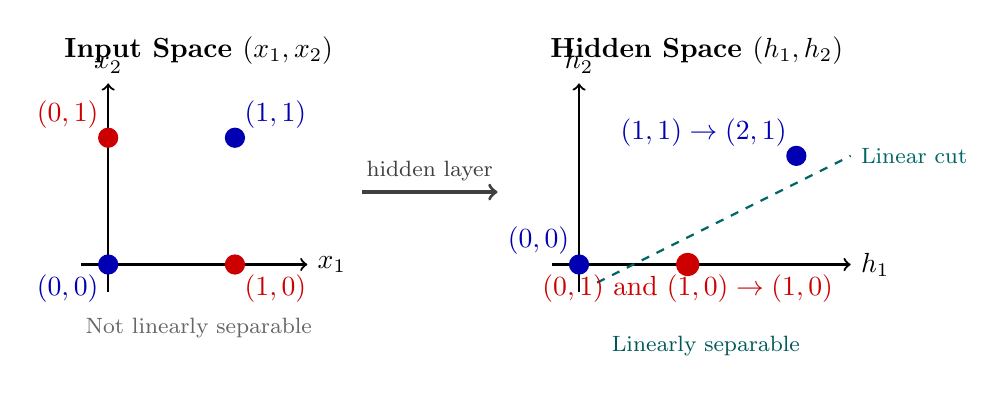
\begin{tikzpicture}[scale=1.15]
        % Left plot: Input Space
        \draw[->, thick] (-0.3,0) -- (2.2,0) node[right] {$x_1$};
        \draw[->, thick] (0,-0.3) -- (0,2.0) node[above] {$x_2$};
        \node[above] at (1.0, 2.1) {\textbf{Input Space $(x_1, x_2)$}};

        % Points in input space
        \filldraw[blue!70!black] (0,0) circle (3pt) node[below left] {$(0,0)$};
        \filldraw[blue!70!black] (1.4,1.4) circle (3pt) node[above right] {$(1,1)$};
        \filldraw[red!80!black] (0,1.4) circle (3pt) node[above left] {$(0,1)$};
        \filldraw[red!80!black] (1.4,0) circle (3pt) node[below right] {$(1,0)$};
        \node[font=\footnotesize, gray!80!black] at (1.0, -0.7) {Not linearly separable};

        % Arrow between spaces
        \draw[->, very thick, darkgray] (2.8, 0.8) -- (4.3, 0.8) node[midway, above, font=\footnotesize] {hidden layer};

        % Right plot: Hidden Space
        \begin{scope}[xshift=5.2cm]
            \draw[->, thick] (-0.3,0) -- (3.0,0) node[right] {$h_1$};
            \draw[->, thick] (0,-0.3) -- (0,2.0) node[above] {$h_2$};
            \node[above] at (1.3, 2.1) {\textbf{Hidden Space $(h_1, h_2)$}};

            % Separating line in hidden space (h_1 - 2 h_2 = 0.5)
            \draw[dashed, thick, teal!80!black] (0.2, -0.2) -- (3.0, 1.2) node[right, font=\footnotesize] {Linear cut};

            % Points in hidden space
            \filldraw[blue!70!black] (0,0) circle (3pt) node[above left] {$(0,0)$};
            \filldraw[red!80!black] (1.2,0) circle (3.5pt) node[below] {$(0,1)$ and $(1,0) \to (1,0)$};
            \filldraw[blue!70!black] (2.4,1.2) circle (3pt) node[above left] {$(1,1) \to (2,1)$};
            \node[font=\footnotesize, teal!70!black] at (1.4, -0.9) {Linearly separable};
        \end{scope}
    \end{tikzpicture}
    \caption{The hidden layer maps both positive points $(0,1)$ and $(1,0)$ onto the same point $(1,0)$ of the hidden space, where a single linear cut separates the two classes.}
    \label{fig:xor_space}
\end{figure}

As Figure~\ref{fig:xor_space} shows, the hidden layer does not bend the output
classifier: it \emph{folds} the input space so that $(0,1)$ and $(1,0)$ land on
the same point $h = (1,0)$, and in the new representation a simple linear cut is
enough.

\begin{note}
    \textbf{Why width helps optimization.} Two ReLU units are enough to represent
    XOR, but training such a network from a random initialization often fails: if a
    unit starts with $z < 0$ on all four points, its gradient is zero everywhere
    and the unit stays dead. With a slightly wider layer (say $8$ or $16$ units)
    gradient descent has many redundant candidates, and nearly every random
    initialization reaches $100\%$ accuracy.
\end{note}

More generally, every hidden unit acts as a \textbf{feature detector}. The score
$z = w^T x + b = \|w\|\|x\|\cos\gamma + b$, where $\gamma$ is the angle between $w$
and $x$, is largest, for a given norm of $x$, when $x$ is aligned with $w$. The
unit therefore works as a template matcher: it responds strongly when a specific
pattern (a stroke, an edge) is present in the input, and stays quiet otherwise. In
a deep network the layers compose these features hierarchically: the first layer
detects simple local patterns, the second combines them into parts or corners, and
the deeper ones assemble abstract concepts.

%==============================================================================
\section{Hidden Units and Activation Functions}
\label{sec:hidden}
%==============================================================================
Every hidden unit computes a pre-activation $z$ and passes it through an
\textbf{activation function} $h = g(z)$. A good hidden activation must meet three
requirements:
\begin{enumerate}
    \item it must be \textbf{non-linear}, so that stacking layers adds expressive
          power;
    \item its derivative $g'(z)$ must stay \textbf{large enough} where $z$
          typically falls, so that gradients can flow backward through many layers;
    \item it must be \textbf{cheap to evaluate}, since $g(z)$ and $g'(z)$ are
          computed millions of times during training.
\end{enumerate}

\paragraph{Saturation and the vanishing gradient problem}
A unit \textbf{saturates} when $|z|$ is so large that it falls in a flat region of
$g$, where $g'(z) \approx 0$. Backpropagation multiplies the error signal by
$g'(z)$, so a saturated unit receives almost no gradient and stops learning.

This is why classical sigmoids are poor hidden activations in deep networks.
Consider a chain of $L = 10$ hidden layers: by the chain rule the gradient of the
loss with respect to a weight $w_1$ of the first layer contains the product of the
slopes of all the activations,
\begin{equation*}
    \frac{\partial \mathcal{L}}{\partial w_1} \propto \prod_{l=1}^{L} g'(z_l)
\end{equation*}
The slope of the logistic sigmoid, $\sigma'(z) = \sigma(z)(1-\sigma(z))$, is at
most $\frac{1}{4}$ (at $z = 0$) and drops below $0.05$ for $|z| > 3$. Even in the
best case, the product of ten such slopes is at most $(1/4)^{10} \approx 10^{-6}$.
The output layer receives a normal gradient and learns quickly, while the first
layers receive a signal a million times weaker and barely move. This exponential
decay of the backward signal is the \textbf{vanishing gradient problem}.

\begin{figure}[!ht]
    \centering
    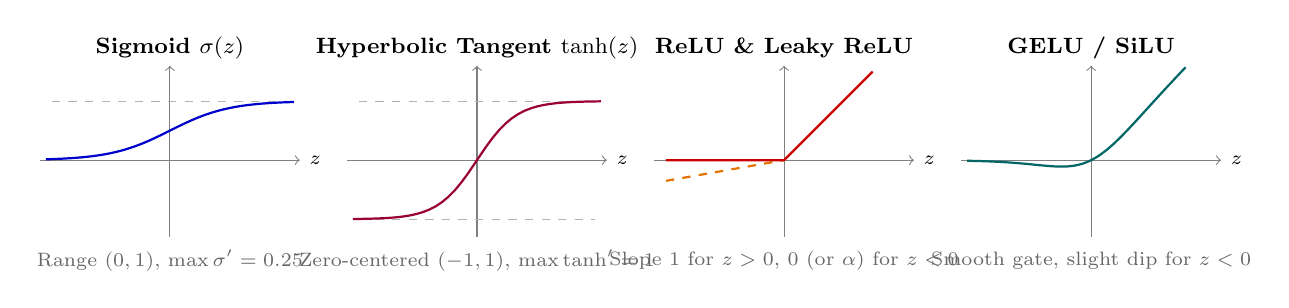
\begin{tikzpicture}[scale=0.75]
        % 1. Sigmoid
        \begin{scope}[xshift=0cm]
            \draw[->, gray] (-2.2,0) -- (2.2,0) node[right, black, font=\scriptsize] {$z$};
            \draw[->, gray] (0,-1.3) -- (0,1.6);
            \draw[dashed, gray!60] (-2,1) -- (2,1);
            \draw[thick, blue!80!black, domain=-2.1:2.1, samples=40] plot (\x, {1/(1+exp(-2*\x))});
            \node[font=\footnotesize\bfseries] at (0, 1.9) {Sigmoid $\sigma(z)$};
            \node[font=\scriptsize, gray!80!black] at (0, -1.7) {Range $(0,1)$, $\max \sigma' = 0.25$};
        \end{scope}

        % 2. Tanh
        \begin{scope}[xshift=5.2cm]
            \draw[->, gray] (-2.2,0) -- (2.2,0) node[right, black, font=\scriptsize] {$z$};
            \draw[->, gray] (0,-1.3) -- (0,1.6);
            \draw[dashed, gray!60] (-2,1) -- (2,1);
            \draw[dashed, gray!60] (-2,-1) -- (2,-1);
            \draw[thick, purple!80!black, domain=-2.1:2.1, samples=40] plot (\x, {tanh(1.5*\x)});
            \node[font=\footnotesize\bfseries] at (0, 1.9) {Hyperbolic Tangent $\tanh(z)$};
            \node[font=\scriptsize, gray!80!black] at (0, -1.7) {Zero-centered $(-1,1)$, $\max \tanh' = 1$};
        \end{scope}

        % 3. ReLU & Leaky ReLU
        \begin{scope}[xshift=10.4cm]
            \draw[->, gray] (-2.2,0) -- (2.2,0) node[right, black, font=\scriptsize] {$z$};
            \draw[->, gray] (0,-1.3) -- (0,1.6);
            \draw[thick, dashed, orange!90!black] (-2.0,-0.35) -- (0,0);
            \draw[thick, red!80!black] (-2.0,0) -- (0,0) -- (1.5,1.5);
            \node[font=\footnotesize\bfseries] at (0, 1.9) {ReLU \& Leaky ReLU};
            \node[font=\scriptsize, gray!80!black] at (0, -1.7) {Slope $1$ for $z>0$, $0$ (or $\alpha$) for $z<0$};
        \end{scope}

        % 4. GELU
        \begin{scope}[xshift=15.6cm]
            \draw[->, gray] (-2.2,0) -- (2.2,0) node[right, black, font=\scriptsize] {$z$};
            \draw[->, gray] (0,-1.3) -- (0,1.6);
            \draw[thick, teal!80!black, domain=-2.1:1.6, samples=50] plot (\x, {\x * (1/(1+exp(-1.702*1.5*\x)))});
            \node[font=\footnotesize\bfseries] at (0, 1.9) {GELU / SiLU};
            \node[font=\scriptsize, gray!80!black] at (0, -1.7) {Smooth gate, slight dip for $z<0$};
        \end{scope}
    \end{tikzpicture}
    \caption{The main hidden activation functions: saturating sigmoids ($\sigma$ and $\tanh$), piecewise linear rectifiers (ReLU and Leaky ReLU) and smooth self-gated units (GELU/SiLU).}
    \label{fig:activations_comparison}
\end{figure}

\subsection{Tanh}
The \textbf{hyperbolic tangent} is a rescaled and shifted logistic sigmoid:
\begin{equation}
    \tanh(z) = 2\sigma(2z) - 1 \in (-1, 1)
\end{equation}
When a bounded, sigmoid-like activation is needed in hidden layers (or in recurrent
networks), $\tanh$ is preferred over the logistic sigmoid for two reasons.
\begin{enumerate}
    \item \textbf{Larger slope near zero}: $\tanh'(0) = 1$ against
          $\sigma'(0) = 0.25$, so gradients survive through more layers while the
          pre-activations stay small.
    \item \textbf{Zero-centered outputs}: the logistic sigmoid only outputs positive
          numbers ($h_j > 0$). Since the gradient of a weight of the next layer is
          $\frac{\partial \mathcal{L}}{\partial w_j} = \delta \cdot h_j$, all the
          weights entering the same neuron get gradients of the \textbf{same sign}
          at every step, and gradient descent zig-zags toward the minimum. Since
          $\tanh(0) = 0$, its outputs take both signs, avoiding the problem.
\end{enumerate}
\begin{note}
    The logistic sigmoid $\sigma(z) \in (0,1)$ belongs to the \textbf{output layer}
    of binary classifiers, where it predicts a probability, while $\tanh(z) \in
    (-1,1)$ is preferred when a saturating activation is needed in the
    \textbf{hidden layers}. Even $\tanh$ saturates for $|z| > 3$, since
    $\tanh'(z) = 1 - \tanh^2(z) \to 0$.
\end{note}

\subsection{Rectified Linear Unit}
The \textbf{Rectified Linear Unit} (ReLU) is the default activation of most
feedforward and convolutional networks:
\begin{equation}
    g(z) = \max(0, z), \qquad g'(z) = \begin{cases} 1 & \text{if } z > 0 \\ 0 & \text{if } z < 0 \end{cases}
\end{equation}
ReLU greatly alleviates the vanishing gradient problem: while a unit is active its
slope is exactly $1$, so it never saturates for positive inputs and the gradient
can cross dozens of layers without shrinking. It is also extremely cheap (a
threshold at zero) and produces \textbf{sparse representations}, since units with
negative pre-activation are switched off. The function is not differentiable at
$z=0$, but in practice optimization simply uses the left or right derivative
(usually $g'(0) = 0$) without any problem.

\paragraph{Dead units: the price of a zero slope}
The main drawback of ReLU is the \textbf{dying ReLU problem}. If the weights and
bias of a unit end up in a region where $z < 0$ for \textbf{every} training
example, the unit outputs $0$ and has derivative $0$ everywhere: it receives no
gradient on any batch, its weights never change again, and the neuron is
permanently dead. This usually comes from a bad initialization (e.g.\ a large
negative bias) or from a \textbf{learning rate that is too large}, whose single
big step pushes the weights deep into the negative half-space. To prevent dead
units we can lower the learning rate, initialize the biases to a small positive
constant (e.g.\ $0.1$), or use a generalization of ReLU that keeps a non-zero slope
for $z < 0$.

\paragraph{ReLU generalizations}
Most piecewise linear variants of ReLU come from one formula:
\begin{equation}
    h_i = g(z_i, \alpha_i) = \max(0, z_i) + \alpha_i \min(0, z_i)
\end{equation}
and differ only in how $\alpha_i$ is chosen:
\begin{itemize}
    \item \textbf{Absolute value rectification}: $\alpha_i = -1$, so $g(z) = |z|$.
          It is used in the early stages of object recognition, where features
          should not change when the polarity is reversed (dark-on-light versus
          light-on-dark edges).
    \item \textbf{Leaky ReLU}: $\alpha_i$ is a small positive constant such as
          $0.01$. The small slope for negative inputs lets even units with $z < 0$
          receive a gradient and recover, which eliminates dead units.
    \item \textbf{Parametric ReLU} (PReLU): $\alpha_i$ is learned by
          backpropagation together with the weights, so each channel or layer can
          adapt its negative slope to the data.
    \item \textbf{Maxout units}: instead of a fixed activation, a maxout unit
          computes $k$ linear filters and returns the maximum:
          \begin{equation}
              g(x) = \max_{j \in \{1, \dots, k\}} \left( w_j^T x + b_j \right)
          \end{equation}
          The unit learns its own activation as a convex, $k$-piece linear function
          (Figure~\ref{fig:Maxout}), which generalizes ReLU, Leaky ReLU and $|z|$.
          The maximum always routes the gradient through the active piece, so
          maxout does not saturate and has no dead units, at the cost of $k$ times
          more parameters per unit.
          \begin{figure}[!ht]
              \centering
              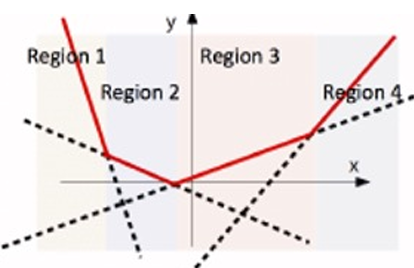
\includegraphics[width=0.5\textwidth]{img/maxout.png}
              \caption{Maxout units}
              \label{fig:Maxout}
          \end{figure}
    \item \textbf{Softplus}: a smooth approximation of ReLU, whose derivative is the
          logistic sigmoid ($\zeta'(z) = \sigma(z)$):
          \begin{equation}
              \zeta(z) = \log(1+e^z)
          \end{equation}
          It was introduced to remove the kink of ReLU at $z=0$, but experiments
          consistently show that plain ReLU trains faster and generalizes better in
          hidden layers. Softplus is mostly useful in output layers, to force a
          positive prediction (for example a variance).
\end{itemize}

\subsection{Modern activation functions: GELU, SiLU and SwiGLU}
Modern architectures, especially Transformers and large language models, replace
the sharp kink of ReLU with smooth \textbf{gated} activations. The idea is to see
ReLU as the product of $z$ and a hard binary gate $\mathbb{I}(z > 0) \in \{0,1\}$,
and to replace the hard gate with a smooth one.
\begin{itemize}
    \item \textbf{GELU} (Gaussian Error Linear Unit) is the standard hidden
          activation of BERT, GPT and Vision Transformers. Its gate is
          $\Phi(z) = P(Z \leq z)$, the cumulative distribution function of a
          standard normal variable $Z \sim \mathcal{N}(0, 1)$:
          \begin{equation}
              \text{GELU}(z) = z \cdot \Phi(z) \approx z \cdot \sigma(1.702 z)
          \end{equation}
          Large positive values pass almost unchanged ($\Phi \to 1$), large negative
          values are blocked ($\Phi \to 0$), and small negative values are partially
          let through. The curve is smooth, with a slight dip below zero (down to
          $-0.17$ near $z \approx -0.75$) that prevents dead units.
    \item \textbf{SiLU} (Sigmoid Linear Unit, or Swish) applies the same principle
          using the logistic sigmoid as the gate; it is used in convolutional
          models such as EfficientNet:
          \begin{equation}
              \text{SiLU}(z) = z \cdot \sigma(z)
          \end{equation}
    \item \textbf{SwiGLU} (Swish-Gated Linear Unit) is used in the feedforward
          blocks of large language models such as LLaMA and PaLM. GELU and SiLU use
          $z$ to gate itself, while SwiGLU \textbf{learns a separate gate} from the
          input $x$, with two parallel projections $W_a$ (content) and $W_b$ (gate):
          \begin{equation}
              h = (W_a^T x + b_a) \odot \text{SiLU}(W_b^T x + b_b)
          \end{equation}
          where $\odot$ is the element-wise product. A SwiGLU block has three weight
          matrices (two projections in, one out) instead of two, so the hidden width
          is usually reduced to $\frac{2}{3}$ of a standard MLP layer to keep the
          number of parameters and FLOPs roughly the same.
\end{itemize}

\subsection{Guidelines for choosing an activation function}
In practice a few rules of thumb are enough:
\begin{itemize}
    \item \textbf{Hidden layers of MLPs and CNNs}: start with \textbf{ReLU} and He
          initialization (Section~\ref{sec:practice}). It is fast, simple and has
          slope $1$ for active units.
    \item \textbf{Many dead units}: switch to \textbf{Leaky ReLU} (or PReLU) and
          lower the learning rate.
    \item \textbf{Transformer feedforward blocks}: use \textbf{GELU} or
          \textbf{SwiGLU}, which have smooth gradients and perform better at scale.
    \item \textbf{Recurrent networks} (RNNs, LSTMs): use the \textbf{sigmoid} for the
          gates, which must lie in $[0,1]$, and \textbf{tanh} for the state updates,
          which must be bounded and zero-centered in $[-1,1]$.
    \item \textbf{Output layer}: never use ReLU at the output of a classifier;
          match the output unit to the target distribution (linear for regression,
          sigmoid for binary classification, softmax for multi-class
          classification).
\end{itemize}

%==============================================================================
\section{Expressive Power and Architecture Design}
\label{sec:expressive}
%==============================================================================
Designing a feedforward network means choosing its \textbf{width} (units per
layer) and its \textbf{depth} (number of layers). To understand why modern
networks prefer depth to sheer width, we first see how a single hidden layer
builds functions.

\subsection{How one hidden layer builds shapes}
In one dimension, a sigmoid unit $\sigma(w(x - c))$ is a soft step that turns on at
$x = c$. The difference of two shifted sigmoids, $\sigma(w(x - a)) - \sigma(w(x - b))$,
steps up at $a$ and down at $b$, producing a localized \textbf{bump}. Likewise,
three ReLU units with output weights $(+1, -2, +1)$ build a triangular \textbf{hat}
(Figure~\ref{fig:hats_and_folding}, left): the first ReLU starts a rising ramp, the
second bends it downward at the peak, and the third flattens it back to zero.
Summing many bumps or hats placed at different locations and scaled by the output
weights, a single hidden layer can trace any continuous curve as a piecewise linear
approximation.

In two or more dimensions each hidden unit defines a \textbf{cut} of the input
space along the hyperplane $w^T x + b = 0$, with high values on one side and low
values on the other. The hidden layer places the cuts and the output layer combines
them like soft logical operators:
\begin{itemize}
    \item the difference of two parallel cuts isolates a \textbf{band};
    \item the sum of two crossing cuts, with a high bias threshold, acts as a
          logical AND and carves out a \textbf{corner};
    \item the difference of two crossing cuts acts as an AND NOT and isolates a
          \textbf{wedge}.
\end{itemize}

\subsection{The Universal Approximation Theorem}
This intuition is formalized by the \textbf{Universal Approximation Theorem}
(Hornik et al., 1989; Cybenko, 1989; Leshno et al., 1993). For any continuous
function $f^*$ on a closed and bounded subset of $\mathbb{R}^d$ and any tolerance
$\varepsilon > 0$, there is a network with \textbf{one hidden layer} of $N$ units
and a linear output layer,
\begin{equation}
    f(x) = \sum_{j=1}^N v_j \, g\left(w_j^T x + b_j\right) + c
\end{equation}
such that $|f(x) - f^*(x)| < \varepsilon$ on the whole domain, as long as the
activation $g$ is continuous and non-polynomial (true for sigmoid, $\tanh$ and
ReLU).

\begin{note}
    \textbf{What the theorem does not say.} It guarantees that a single hidden layer
    \emph{can} represent any continuous function, but with three caveats:
    \begin{enumerate}
        \item \textbf{the width can be exponential}: in $d$ dimensions, placing local
              bumps or kinks on a grid to match an arbitrary function may require
              $N \sim \mathcal{O}(\varepsilon^{-d})$ units;
        \item \textbf{no optimization guarantee}: the right weights exist, but
              gradient descent is not guaranteed to find them;
        \item \textbf{no generalization guarantee}: a huge single layer may simply
              memorize the training points and generalize poorly.
    \end{enumerate}
\end{note}

\subsection{Why depth helps: composition and space folding}
Adding units to one layer \textbf{adds} linear pieces (kinks), while stacking
layers \textbf{composes} functions and \textbf{multiplies} the pieces.

Take a symmetric ``tent'' function $t(x)$ on $[0,1]$ built with $2$ ReLU units: it
rises from $0$ to $1$ at $x = 0.5$ and falls back to $0$ at $x = 1$, so it has $2$
linear pieces. If its output is fed into an identical tent layer, the composition
$t(t(x))$ folds the interval in half before applying the tent again, and has
$2 \times 2 = 4$ pieces. Stacking $L$ layers uses only $2L$ units but produces
$2^L$ linear pieces (Figure~\ref{fig:hats_and_folding}, right), a function that a
single layer would need about $2^L$ units to build. More generally
(Mont\'ufar et al., 2014), the number of linear regions of a ReLU network grows
\textbf{polynomially with the width} but \textbf{exponentially with the depth}.

\begin{figure}[!ht]
    \centering
    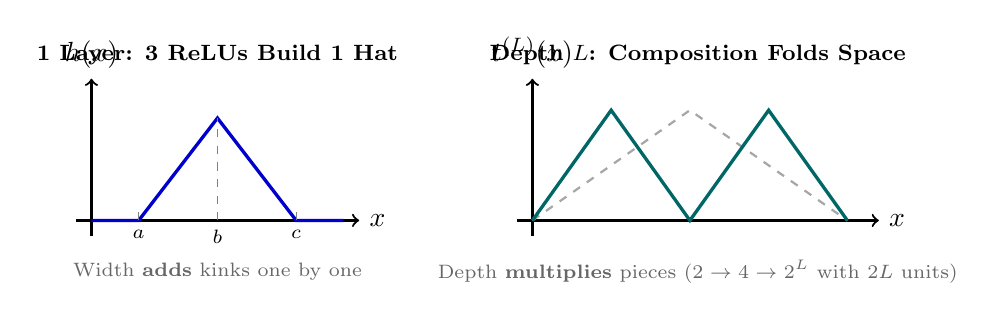
\begin{tikzpicture}[scale=1.0]
        % Left: 3 ReLUs make a hat
        \begin{scope}[xshift=0cm]
            \draw[->, thick] (-0.2,0) -- (3.4,0) node[right] {$x$};
            \draw[->, thick] (0,-0.2) -- (0,1.8) node[above] {$h(x)$};
            \draw[very thick, blue!80!black] (0,0) -- (0.6,0) -- (1.6,1.3) -- (2.6,0) -- (3.2,0);
            \draw[dashed, gray] (0.6,0) node[below, black, font=\scriptsize] {$a$} -- (0.6, 0.2);
            \draw[dashed, gray] (1.6,0) node[below, black, font=\scriptsize] {$b$} -- (1.6, 1.3);
            \draw[dashed, gray] (2.6,0) node[below, black, font=\scriptsize] {$c$} -- (2.6, 0.2);
            \node[font=\footnotesize\bfseries] at (1.6, 2.1) {1 Layer: 3 ReLUs Build 1 Hat};
            \node[font=\scriptsize, gray!80!black] at (1.6, -0.65) {Width \textbf{adds} kinks one by one};
        \end{scope}

        % Right: Composition multiplies pieces
        \begin{scope}[xshift=5.6cm]
            \draw[->, thick] (-0.2,0) -- (4.4,0) node[right] {$x$};
            \draw[->, thick] (0,-0.2) -- (0,1.8) node[above] {$t^{(L)}(x)$};
            % L=1 (dashed)
            \draw[dashed, thick, gray!70] (0,0) -- (2.0,1.4) -- (4.0,0);
            % L=2 (solid)
            \draw[very thick, teal!80!black] (0,0) -- (1.0,1.4) -- (2.0,0) -- (3.0,1.4) -- (4.0,0);
            \node[font=\footnotesize\bfseries] at (2.1, 2.1) {Depth $L$: Composition Folds Space};
            \node[font=\scriptsize, gray!80!black] at (2.1, -0.65) {Depth \textbf{multiplies} pieces ($2 \to 4 \to 2^L$ with $2L$ units)};
        \end{scope}
    \end{tikzpicture}
    \caption{Left: three ReLU units of a single layer combine into a localized ``hat''. Right: composing a 2-ReLU ``tent'' over $L$ layers folds the input space again and again, doubling the number of linear segments at each layer.}
    \label{fig:hats_and_folding}
\end{figure}

Geometrically, each layer with a folding activation (a tent, or $|z|$) folds the
input space like a sheet of paper along a hyperplane, so whatever the following
layers learn is automatically replicated on both halves of the fold ($2^L$ copies
after $L$ layers). Choosing a deep architecture therefore encodes a strong prior:
the target function is a \textbf{hierarchical composition of simpler steps}. This
is why deep networks generalize much better on real tasks than shallow ones with
the same number of parameters.

\subsection{Beyond the dense chain: connectivity and skip connections}
A standard MLP connects every unit of layer $l-1$ to every unit of layer $l$,
without assumptions on the structure of the input. When the data have known
symmetries we specialize the connectivity: \textbf{convolutional networks} (CNNs)
use local connections and share weights across space for images, while
\textbf{recurrent networks} (RNNs) share weights across time for sequences.

Finally, with very deep networks ($30$ to $100+$ layers) training can degrade even
with ReLU and a good initialization. Modern architectures solve this with
\textbf{skip (residual) connections}:
\begin{equation}
    h^{(l+1)} = h^{(l)} + F(h^{(l)})
\end{equation}
Instead of re-learning the whole representation, the layer only learns an additive
correction $F(h^{(l)})$ to its input. In backpropagation the identity path
$+h^{(l)}$ is a direct highway along which gradients flow across many layers
unimpeded.

%==============================================================================
\section{Cost Functions and Output Units}
\label{sec:loss-output}
%==============================================================================
Now that we know how the network computes a prediction, we need to measure how good
it is, and to make sure that its last layer produces something the loss can
evaluate. The two choices are tightly coupled: the loss comes from the probability
distribution we assume for the target, and the output unit produces the parameters
of that distribution.

\subsection{Loss and cost}
\begin{definition}[\textbf{Loss function}]
    A \textbf{loss function} $\mathcal{L}(\hat{y}, y)$ maps the prediction of the
    model on a single data point and its true target to a real number that
    quantifies the error on that example.
\end{definition}
\begin{definition}[\textbf{Cost function}]
    A \textbf{cost function} $J(\theta)$ is the average loss over the whole
    training set (often combined with a regularization term). It is the overall
    objective that the learning algorithm seeks to minimize.
\end{definition}

\subsection{Maximum likelihood: where the losses come from}
Rather than picking a loss arbitrarily, deep learning derives it from one
principle, \textbf{Maximum Likelihood Estimation} (MLE). Instead of seeing the
network as outputting a bare number, we see it as predicting the parameters of a
conditional distribution $p_{\text{model}}(y \mid x; \theta)$ of the target $y$
given the input $x$.

MLE looks for the parameters that give the highest probability to the observed
targets. Maximizing the product of the probabilities of $N$ independent examples is
equivalent to minimizing the average \textbf{Negative Log-Likelihood} (NLL), which
is also the \textbf{cross-entropy} between the empirical data distribution and the
model distribution:
\begin{equation}
    J(\theta) = -\frac{1}{N} \sum_{i=1}^N \log p_{\text{model}}(y_i \mid x_i; \theta)
\end{equation}
Every standard loss for regression and classification follows once we choose the
family of $p_{\text{model}}$.

\subsection{Regression losses}
\begin{itemize}
    \item \textbf{Mean Squared Error} (MSE) comes from MLE by assuming that the
          target is the network output plus Gaussian noise,
          $p_{\text{model}}(y \mid x) = \mathcal{N}(y; \hat{y}(x), \sigma^2)$:
          \begin{equation}
              \mathcal{L} = \frac{1}{N} \sum_{i=1}^N (y_i - \hat{y}_i)^2
          \end{equation}
          Squaring means that doubling the error quadruples the penalty, so large
          outliers dominate the gradient. The optimal predictor of the MSE is the
          \textbf{conditional mean} $\hat{y}^*(x) = \mathbb{E}[y \mid x]$.
    \item \textbf{Mean Absolute Error} (MAE) comes from assuming a heavy-tailed
          \textbf{Laplace} distribution around $\hat{y}(x)$:
          \begin{equation}
              \mathcal{L} = \frac{1}{N} \sum_{i=1}^N |y_i - \hat{y}_i|
          \end{equation}
          The gradient with respect to $\hat{y}_i$ is $\pm 1$ whatever the size of
          the error, so large errors are not amplified and the loss is robust to
          outliers. The optimal predictor is the \textbf{conditional median}
          $\hat{y}^*(x) = \text{median}(y \mid x)$. The price is a derivative that
          is discontinuous at $y_i = \hat{y}_i$.
    \item \textbf{Huber loss} combines the best of the two to handle outliers
          smoothly: quadratic for small errors, which gives a smooth gradient near
          zero, and linear for large errors, which keeps outliers from hijacking
          the training:
          \begin{equation}
              \mathcal{L} = \frac{1}{N} \sum_{i=1}^N \begin{cases}
                  \frac{1}{2}(y_i - \hat{y}_i)^2                  & \text{if } |y_i - \hat{y}_i| \leq \delta \\
                  \delta |y_i - \hat{y}_i| - \frac{1}{2} \delta^2 & \text{otherwise}
              \end{cases}
          \end{equation}
\end{itemize}

\subsection{Classification losses}
\begin{itemize}
    \item \textbf{Binary cross-entropy} (log-loss) comes from a \textbf{Bernoulli}
          distribution with $y_i \in \{0, 1\}$ and predicted probability
          $\hat{y}_i = P(y_i = 1 \mid x_i)$:
          \begin{equation}
              \mathcal{L} = - \frac{1}{N} \sum_{i=1}^N \Big( y_i \log(\hat{y}_i) + (1-y_i) \log(1-\hat{y}_i) \Big)
          \end{equation}
          If the model is confident and right ($\hat{y}_i \to y_i$) the loss goes to
          $0$; if it is confident and wrong ($\hat{y}_i \to 1 - y_i$) the loss
          blows up to infinity, so overconfident mistakes are punished heavily.
    \item \textbf{Categorical cross-entropy} comes from a \textbf{Categorical}
          distribution over $k$ mutually exclusive classes. If $y_{i,c} \in \{0,1\}$
          is the one-hot indicator of the true class of example $i$:
          \begin{equation}
              \mathcal{L} = - \frac{1}{N} \sum_{i=1}^N \sum_{c=1}^k y_{i,c} \log(\hat{y}_{i,c}) = - \frac{1}{N} \sum_{i=1}^N \log(\hat{y}_{i, y_i})
          \end{equation}
          Only the true class has a non-zero indicator, so the loss of each example
          depends only on the probability $\hat{y}_{i, y_i}$ assigned to the correct
          class.
    \item \textbf{Hinge loss} is a margin-based alternative for binary
          classification, with labels $y_i \in \{-1, +1\}$ and $z_i$ the raw linear
          score:
          \begin{equation}
              \mathcal{L} = \frac{1}{N} \sum_{i=1}^N \max(0, 1 - y_i z_i)
          \end{equation}
          The product $y_i z_i$ is the \textbf{margin}, positive when the sign of
          the prediction is correct. Cross-entropy never reaches zero and keeps
          pushing the logits to grow, whereas the hinge loss is exactly $0$ when
          $y_i z_i \geq 1$: once an example is correctly classified beyond the
          safety margin, it stops contributing to the gradient.
\end{itemize}
\begin{note}
    Any custom loss can be used in deep learning, as long as it is differentiable
    almost everywhere, so that it stays compatible with gradient-based
    optimization.
\end{note}

\subsection{Output units}
\label{sec:output-units}
The hidden layers extract a feature vector $h$. The \textbf{output unit} is the
last layer: it transforms the logits $z = W^T h + b$ into the parameters of the
conditional distribution $p_{\text{model}}(y \mid x)$ chosen above.

\subsubsection{Linear output unit}
The linear unit returns the affine transformation directly:
\begin{equation}
    \hat{y} = W^T h + b
\end{equation}
It is used in regression, where $\hat{y} \in \mathbb{R}$ is the mean of a
conditional Gaussian $\mathcal{N}(y; \hat{y}, \sigma^2)$, and maximum likelihood
reduces to minimizing the MSE. Its great advantage is that its slope is always $1$:
it \textbf{never saturates}, so the gradient $\hat{y} - y$ reaches the network
without shrinking, however far the prediction is from the target.

If we also want the network to predict its own, input-dependent uncertainty
(\emph{heteroscedastic} regression), the output layer emits two values: the mean
$\hat{y}(x)$ and a raw value $v(x)$, which goes through a softplus,
$s^2(x) = \log(1 + e^{v(x)})$, so that the predicted variance is always strictly
positive.

\subsubsection{Sigmoid output unit}
The sigmoid unit is used for \textbf{binary classification} ($y \in \{0, 1\}$) and
models a Bernoulli distribution. From one scalar logit $z = w^T h + b$ it produces
a valid probability $\hat{y} = \sigma(z) \in (0,1)$. The logit is the
\textbf{log-odds} of the positive class, since
$\log \frac{\hat{y}}{1 - \hat{y}} = z$: we have $\hat{y} = 0.5$ when $z = 0$,
$\hat{y} > 0.5$ when $z > 0$ and $\hat{y} < 0.5$ when $z < 0$.

\begin{note}
    \textbf{Why a sigmoid output is paired with cross-entropy and not with MSE.}
    Suppose the true label is $y = 1$, but the model is confidently wrong, with
    $z = -5$ ($\hat{y} \approx 0.007$). The sigmoid is deep in its flat region,
    where $\sigma'(z) = \hat{y}(1 - \hat{y}) \approx 0.007$.
    \begin{itemize}
        \item With the \textbf{squared error} $\mathcal{L} = (\hat{y} - y)^2$ the
              chain rule multiplies the error by $\sigma'(z)$, and the gradient is
              tiny: the network barely learns exactly when it is most wrong.
        \item With the \textbf{binary cross-entropy}
              $\mathcal{L} = -y\log\hat{y} - (1-y)\log(1-\hat{y}) = \log(1 + e^{(1-2y)z})$
              the logarithm undoes the exponential of the sigmoid, and the gradient
              with respect to the logit simplifies to
              \begin{equation*}
                  \frac{\partial \mathcal{L}}{\partial z} = \hat{y} - y
              \end{equation*}
              With $y = 1$ and $\hat{y} \approx 0$ the gradient is $-1$: strong, and
              it never saturates when the model is wrong. It flattens out only as
              $\hat{y} \to y$, when the model is already right.
    \end{itemize}
\end{note}

For \textbf{multi-label classification}, where an input can belong to several
non-exclusive categories at the same time (e.g.\ an image tagged ``outdoor'' and
``dog''), we use $k$ independent sigmoid units trained with the sum of $k$ binary
cross-entropies.

\subsubsection{Softmax output unit}
The softmax unit generalizes the sigmoid to \textbf{multi-class classification}
with $k$ mutually exclusive classes, modeling a Categorical distribution. A linear
layer produces $k$ un-normalized logits $z \in \mathbb{R}^k$, and the softmax
exponentiates and normalizes them, so that they are positive and sum to $1$.

Combined with categorical cross-entropy, the negative log-likelihood of an example
of true class $y$ is
\begin{equation}
    \mathcal{L}(z, y) = -\log \text{softmax}(z)_y = -z_y + \log \sum_{j=1}^k e^{z_j}
\end{equation}
which shows how the learning works. The first term, $-z_y$, pushes the logit of the
correct class \textbf{up}. The second, $\log \sum_j e^{z_j} \approx \max_j z_j$,
pushes all the logits \textbf{down}, in proportion to their predicted probability
$\hat{y}_j$ (hardest on the strongest competitor). As in the binary case, the $\log$
cancels the $\exp$ and the gradient is the clean vector
$\nabla_z \mathcal{L} = \text{softmax}(z) - e_y$, which does not vanish when the
prediction is wrong.

\paragraph{Shift invariance and numerical stability}
Adding the same constant $c$ to all the logits does not change the probabilities:
\begin{equation*}
    \text{softmax}(z + c)_i = \frac{e^{z_i + c}}{\sum_j e^{z_j + c}} = \frac{e^c e^{z_i}}{e^c \sum_j e^{z_j}} = \text{softmax}(z)_i
\end{equation*}
On a computer, $e^{z_i}$ \textbf{overflows} to $\infty$ if $z_i$ is large and
positive (e.g.\ $1000$), and all the exponentials \textbf{underflow} to $0$ (giving
$0/0$) if all the $z_i$ are large and negative. The standard solution is to subtract
$c = \max_j z_j$ before exponentiating:
\begin{equation}
    \text{softmax}(z) = \text{softmax}\big(z - \max_j z_j\big)
\end{equation}
The largest exponent is then $e^0 = 1$ and all the others are in $[0, 1]$, so there
is neither overflow nor division by zero.

\subsubsection{Gaussian Mixtures output unit}
In some regression problems, especially inverse ones such as finding the joint
angles of a robot arm that reach a given hand position, the same input $x$ admits
\textbf{several valid answers} $y$: the problem is \textbf{multimodal}. A single
linear output trained with MSE is the wrong tool: it predicts the conditional mean
$\mathbb{E}[y \mid x]$, which averages the valid branches and lands between them,
possibly on an answer that is not valid at all.

To capture several peaks for the same $x$, a \textbf{Mixture Density Network} (MDN)
uses a \textbf{Gaussian Mixture Model} (GMM) as output distribution:
\begin{equation}
    p(y \mid x) = \sum_{i=1}^K \pi_i(x) \, \mathcal{N}\big(y; \mu^{(i)}(x), \Sigma^{(i)}(x)\big)
\end{equation}
It is trained by minimizing the negative log-likelihood $-\log p(y \mid x)$. The
last layer emits three groups of outputs, each passed through a transformation that
enforces its constraint:
\begin{itemize}
    \item the \textbf{mixture weights} $\pi_i(x) = p(c=i \mid x)$, the probability of
          selecting the $i$-th Gaussian. They must be positive and sum to $1$, so
          they use a \textbf{softmax};
    \item the \textbf{means} $\mu^{(i)}(x)$, the center of each branch. They are
          unconstrained, so they use \textbf{linear} units;
    \item the \textbf{variances/covariances} $\Sigma^{(i)}(x)$, the spread around each
          branch. They must be strictly positive, so the raw outputs go through a
          \textbf{softplus} ($\log(1+e^v)$) or an exponential ($e^v$).
\end{itemize}

%==============================================================================
\section{Gradient-Based Optimization}
\label{sec:optimization}
%==============================================================================
\subsection{The objective and gradient descent}
Over the $n$ training samples, the objective (cost) function that measures the
discrepancy between the learned function and the true targets is
\begin{equation}
    J(\theta) = \frac{1}{n} \sum_{i=1}^n \mathcal{L}(x_i, y_i, \theta)
\end{equation}
and training looks for the parameters that minimize it:
\begin{equation}
    \hat{\theta} = \argmin_{\theta} J(\theta) = \argmin_{\theta} \frac{1}{n}
    \sum_{i=1}^n \mathcal{L}(x_i, y_i, \theta)
\end{equation}

To minimize $J$ we compute its \textbf{gradient} $\nabla_\theta J(\theta)$, the
vector whose $i$-th component is the partial derivative
$\frac{\partial J}{\partial \theta_i}$, i.e.\ how the cost changes when only
$\theta_i$ is varied slightly. The gradient points in the direction of steepest
increase, so \textbf{gradient descent} moves in the opposite direction:
\begin{equation}
    \theta' = \theta - \eta \nabla_\theta J(\theta)
\end{equation}
where $\eta > 0$ is the \textbf{learning rate}, which controls the size of the step.
Gradient descent has converged when every component of the gradient is zero.

The best learning rate may change during training. A practical strategy is to start
with a moderately large $\eta$, which makes fast progress at the beginning and
helps to leave shallow regions, and then to decrease it gradually, so that the
parameters can settle near a minimum.

\begin{note}
    \textbf{Convex and non-convex landscapes.} For linear models $J(\theta)$ is a
    convex bowl with a single global minimum, which gradient descent reaches from
    any starting point. In deep networks the non-linear activations of the hidden
    layers make $J(\theta)$ \textbf{non-convex}: the landscape has many local minima
    and saddle points, and the solution we reach depends on the initialization of
    $\theta$. Since non-convex objectives have no closed-form solution, we rely on
    iterative numerical optimization.
\end{note}

\subsection{Regularization}
To reduce the risk of overfitting we can add a \textbf{regularization term} to the
objective:
\begin{equation}
    \hat{\theta} = \argmin_{\theta} \frac{1}{n} \sum_{i=1}^n \mathcal{L}(x_i, y_i, \theta)
    + \lambda R(\theta)
\end{equation}
where $R(\theta)$ penalizes the complexity of the model and $\lambda$ is a
hyperparameter that balances fitting the data against keeping the model simple.
Regularization can also be applied implicitly, through architectural or data
choices, such as randomly disabling units or connections (dropout) or injecting
noise into the inputs.
\begin{note}
    Networks with smaller weights tend to generalize better than networks with
    larger weights, because small perturbations or noise in the input produce much
    smaller fluctuations in the output.
\end{note}

\subsection{Minibatch Stochastic Gradient Descent}
Computing the exact gradient on the whole dataset (\textbf{full-batch} gradient
descent) costs $\mathcal{O}(n)$ per step, which is prohibitively slow when $n$
ranges from thousands to billions of examples. \textbf{Stochastic Gradient Descent}
(SGD) removes the bottleneck by estimating the gradient on a small random subset of
the data at each step.

At one extreme, \textbf{online learning} ($m = 1$) updates the weights after a
single example: updates are immediate, but the estimate is very noisy and does not
exploit the parallelism of GPUs. In practice we use \textbf{mini-batch SGD}: we draw
a random subset of $m$ examples (typically $32 \leq m \leq 512$) and compute their
average gradient,
\begin{equation}
    g = \frac{1}{m} \sum_{i = 1}^{m} \nabla_{\theta} \mathcal{L}(x_i, y_i, \theta)
\end{equation}
followed by the update
\begin{equation}
    \theta = \theta - \eta g
\end{equation}
A complete pass over the $n$ training examples ($n/m$ mini-batch steps) is called an
\textbf{epoch}.

Why do small mini-batches work so well? The mini-batch gradient $g$ is an
\textbf{unbiased} estimator of the true gradient,
$\mathbb{E}[g] = \nabla_\theta J(\theta)$, and its standard deviation (the gradient
noise) shrinks as $1/\sqrt{m}$. This square-root law means diminishing returns for
large batches: using $100\times$ more examples per step costs $100\times$ more
computation but reduces the noise only by $10\times$. Taking many fast, slightly
noisy steps with a moderate batch converges much faster in wall-clock time than
taking one slow, exact step. The choice of $m$ is therefore a trade-off: larger
batches give more accurate gradients but slower convergence, smaller batches give
noisier gradients but faster convergence.

%==============================================================================
\section{Backpropagation}
\label{sec:backprop}
%==============================================================================
Gradient descent needs the gradient of the loss with respect to every weight and
bias of the network. \textbf{Backpropagation} computes it efficiently by applying
the \textbf{chain rule of calculus} recursively, from the output layer back to the
input layer, reusing at each step what was computed for the layer above.

\subsection{Chain rule}
If $\mathcal{L}$ depends on $z$, which in turn depends on $w$, then
\begin{equation}
    \frac{\partial \mathcal{L}}{\partial w} = \frac{\partial \mathcal{L}}{\partial z} \cdot \frac{\partial z}{\partial w}
\end{equation}

\subsection{The backward pass step by step}
We follow the computation on a network with one hidden layer and a sigmoid output
unit, where
$z^{(1)} = W^{(1)T}x + b^{(1)}$, $h = g(z^{(1)})$, $z = w^{(2)T} h + b^{(2)}$ and
$\hat{y} = \sigma(z)$.

\paragraph{1. Output layer.} First we compute how the loss changes with respect to
the logit $z$:
\begin{equation}
    \frac{\partial \mathcal{L}}{\partial z} = \frac{\partial \mathcal{L}}{\partial \hat{y}} \cdot \frac{\partial \hat{y}}{\partial z}
\end{equation}
With a sigmoid output $\hat{y} = \sigma(z)$ and the binary cross-entropy
$\mathcal{L} = -y \log(\hat{y}) - (1-y)\log(1-\hat{y})$, using
$\sigma'(z) = \sigma(z)(1-\sigma(z)) = \hat{y}(1-\hat{y})$, everything simplifies to
\begin{equation}
    \frac{\partial \mathcal{L}}{\partial z} = \hat{y} - y
\end{equation}

\paragraph{2. Output weights and bias.} Since
$z = \sum_j w_j^{(2)} h_j + b^{(2)}$, we have $\frac{\partial z}{\partial w_j^{(2)}} = h_j$
and $\frac{\partial z}{\partial b^{(2)}} = 1$, so the chain rule gives
\begin{equation}
    \frac{\partial \mathcal{L}}{\partial w^{(2)}} = \frac{\partial \mathcal{L}}{\partial z} \cdot h \quad \text{and} \quad \frac{\partial \mathcal{L}}{\partial b^{(2)}} = \frac{\partial \mathcal{L}}{\partial z}
\end{equation}

\paragraph{3. Back to the hidden layer.} To update $W^{(1)}$ and $b^{(1)}$ the error
signal travels backward, first through the output weights and then through the
derivative of the hidden activation $g'\left(z^{(1)}\right)$:
\begin{equation}
    \frac{\partial \mathcal{L}}{\partial h} = \frac{\partial \mathcal{L}}{\partial z} \cdot w^{(2)}
\end{equation}
\begin{equation}
    \delta^{(1)} = \frac{\partial \mathcal{L}}{\partial z^{(1)}} = \frac{\partial \mathcal{L}}{\partial h} \odot g'\left(z^{(1)}\right)
\end{equation}
where $\odot$ is the element-wise (Hadamard) product. For a ReLU hidden layer
($h = \max\{0, z^{(1)}\}$), $g'(z_j^{(1)}) = 1$ if $z_j^{(1)} > 0$ and $0$ if
$z_j^{(1)} \leq 0$.

\paragraph{4. First layer parameters.} Finally,
\begin{equation}
    \frac{\partial \mathcal{L}}{\partial W^{(1)}} = x \cdot \left(\delta^{(1)}\right)^T \quad \text{and} \quad \frac{\partial \mathcal{L}}{\partial b^{(1)}} = \delta^{(1)}
\end{equation}

\begin{note}
    \textbf{Inactive ReLU units receive no update.} The gradient of an output weight
    is proportional to the activation of its hidden unit,
    $\frac{\partial \mathcal{L}}{\partial w_j^{(2)}} = \frac{\partial \mathcal{L}}{\partial z} \cdot h_j$.
    A neuron that is inactive in the forward pass
    ($z_j^{(1)} \leq 0 \implies h_j = 0$) therefore produces a zero gradient, and its
    outgoing weight $w_j^{(2)}$ is not updated. The same holds for its incoming
    weights, since $g'(z_j^{(1)}) = 0$.
\end{note}

%==============================================================================
\section{Training in Practice}
\label{sec:practice}
%==============================================================================
\subsection{Weight initialization}
Activations decide how the signal flows, but the initialization of weights and
biases is just as important: it keeps the signal from exploding or vanishing across
the layers and makes training stable. It follows three ideas.

\paragraph{Avoid saturation} A unit saturates when its pre-activation $|z|$ is too
large (Section~\ref{sec:hidden}), and then it receives almost no gradient. To avoid
saturation at the start of training, inputs should be standardized and the initial
weights kept small.

\paragraph{Break the symmetry} Weights must \textbf{never} be initialized to the
same value (such as all zeros). If all the weights of a layer are equal, every unit
computes the same output, receives the same gradient and undergoes the same update:
the units remain identical clones forever, and a layer of $512$ units behaves like a
single neuron. Drawing the weights at random breaks the symmetry. \textbf{Biases},
instead, can safely start at $0$ (which also lets us discover dead neurons), or at a
small positive value such as $0.1$ for ReLU units, so that they do not start in the
inactive region $z < 0$.

\paragraph{Preserve the scale} The scale of the random weights must preserve the
variance of the activations going forward and of the gradients going backward across
all the $L$ layers: if the weights are too large, activations explode exponentially
with depth; if they are too small, they shrink to zero. Two standard schemes, which
sample from a normal distribution with zero mean and a variance that depends on the
number of neurons $n^{[l]}$ of the layers, correspond to the two main families of
activations:
\begin{itemize}
    \item \textbf{Glorot (Xavier) initialization} is designed for symmetric,
          zero-centered activations such as $\tanh$ (and the sigmoid), which are
          roughly linear with slope $1$ around the origin. It is a compromise
          between preserving the forward scale ($1/n^{[l-1]}$) and the backward
          scale ($1/n^{[l]}$):
          \begin{equation*}
              W^{[l]} \sim \mathcal{N}\left(0, \frac{2}{n^{[l-1]} + n^{[l]}}\right)
          \end{equation*}
    \item \textbf{He (Kaiming) initialization} is designed for \textbf{ReLU}.
          Since ReLU zeroes all the negative inputs, it silences about half of the
          units of each layer and halves the variance of the signal; the factor $2$
          in the numerator compensates for the lost half:
          \begin{equation*}
              W^{[l]} \sim \mathcal{N}\left(0, \frac{2}{n^{[l-1]}}\right)
          \end{equation*}
\end{itemize}
A good initialization keeps activations and gradients well scaled from the very
first step, which allows fast and reliable convergence.

\subsection{The whole training procedure}
We can now put all the pieces together. The weights are randomly initialized. Then,
for each training example $(x, y)$ (in practice, for each mini-batch), the network
computes a forward pass to obtain $\hat{y} = f(x; \theta)$; the error
$\mathcal{L}(\hat{y}, y)$ is evaluated; backpropagation computes the gradient; and
all the weights are adjusted in the direction that reduces the error. Repeating this
over many epochs gradually minimizes the cost function.

\section{Regularization}
\textbf{Regularization} is a crucial technique in deep learning to prevent
\textit{overfitting}, which occurs when a model performs well on training data
but poorly on unseen data. Regularization strategies aim to reduce the model's
variance at the cost of slightly increasing its bias. This trade-off results in
a model that generalizes better to new data. Below we will list some of the
regularization techniques that we will go to see:
\begin{itemize}
    \item Parameters norm penalties;
    \item Dataset augmentation;
    \item Noise robustness;
    \item Early stopping;
    \item Parameter tying and parameter sharing;
    \item Multitask learning;
    \item Bagging and other ensemble methods;
    \item Dropout;
    \item Adversarial training;
\end{itemize}

We need to have a model that is capable to generalize on unseen data, so we have
to find the right trade-off in order to avoid overfitting and underfitting.

In the context of deep learning, most regularization strategies are based on
\textbf{regularizing estimators}. This is done through reducing \textbf{variance}
at the expense of increasing the \textbf{bias} of the estimator.
\begin{note}
    A good estimator is one that decreases the variance without increasing too
    much the bias.
\end{note}

When we are working with deep learning to solve complex tasks, we can encounter
different problems. This can increase the complexity of the model and the risk of
overfitting. In this case, we can find the best large model and in the end apply
a regularization process to reduce the complexity of the model and improve the
generalization.

The concept of regularization in machine learning and deep learning is to create
models that not only minimize the loss function but also manage the variability
and generalization capability of the model. To accomplish this, we can employ the
following strategies:
\begin{itemize}
    \item \textbf{Directly}: incorporates prior knowledge or expresses a generic
          preference for simpler models by directly altering the model or its
          training process. This is implemented by changing constraints, adding
          restrictions on the parameter values or changing objective function.
          The constraints serve to penalize certain values of the parameters;
    \item \textbf{Undirectly}: this method does not manipulate the model directly
          but alters the training process or data to enhance generalization. This
          can be done using technique such as data augmentation, introducing noise
          in the training data or using ensemble methods.
\end{itemize}
\subsection{Regularization strategies}
\subsubsection{Parameters Norm Penalties}
The most traditional form of regularization consists in adding a penalty term to
the loss function, encouraging smaller or sparser parameter values. It can be
formulated as:
\begin{equation}
    \hat{J}(\theta) = J(\theta) + \alpha \Omega(\theta)
\end{equation}
where $\alpha \in [0, \infty)$ is a hyperparameter that regulates the contribution
of the norm penalties, and $\Omega(\theta)$ is the penalty term. This parameter
can change for each layer.

Since we have added a penalty term, the optimizer will try to minimize the loss
function and at the same time it decreases some measure of the size of the
parameters $\theta$. It affects only a subset of parameters.

$\Omega$ usually penalizes only the weights ($W$) of the affine transformation
at each layer, not the bias ($b$).

This method can be implemented using different norms, here we can see some of them:
\begin{itemize}
    \item \textbf{Sum of the weights} or \textbf{$L_1$ Norm} ($L_1$): Promotes
          sparsity pushing all values to $0$ penalizing small weights more than big one.
          \begin{equation}
              \Omega(w) = \sum_{w_j}|w_j| = \|w\|_1
          \end{equation}
    \item \textbf{Sum of the squared weights} or \textbf{$L_2$ Norm} ($L_2$):
          penalizes larger weights, encouraging smoothness:
          \begin{equation}
              \Omega(w) = \sum_{w_j}|w_j|^2 = \|w\|_2
          \end{equation}
    \item \textbf{$p$-norm} ($L_p$): for $p < 2$ encourage sparser vector, while
          larger values of $p$ discourage large weights more:
          \begin{equation}
              \Omega(w) = \sqrt[p]{\sum_{w_j}|w_j|^p} = \|w\|_p
          \end{equation}
          In general, all the $p-$norms are used to penalize large weights more
          than small ones.
\end{itemize}

The effect of the $L_2$ norm is to shrinks weights on features that add noise to
the model (feature with high variance but low covariance with target), while
$L_1$ norm provides a solution that is sparse. This property can be seen as a
features selection mechanism.
\begin{note}
    Using $L_2$ negative and positive weights moves towards 0 depending on the
    magnitude of the weights, while using $L_1$ negative and positive weights
    moves towards 0 regardless of magnitude.
\end{note}

Another improve that we can add to the previous model are constraints related to
regularization term, for example, if we consider the following loss function:
\begin{equation}
    \hat{J}(\theta) = J(\theta) + \alpha \Omega(\theta)
\end{equation}
we can add a constraint to the regularization term as follows:
\begin{equation}
    \Omega(\theta) \le k
\end{equation}
where $k$ is a small value. In this way the optimization problem changed because
we have to consider also the upper-bound of regularization term.

To solve this problem, we can construct a generalize \textbf{Lagrange function},
consisting of the original objective function plus a set of penalties. Each
penalty is a product between a coefficient, called a Lagrange multiplier ($\alpha$),
and a function representing whether the constraint is satisfied.
\begin{equation}
    \mathcal{L}(\theta, \alpha; X,y) = J(w;X,y)+ \alpha(\Omega(\theta)-k)
\end{equation}
Formally the optimization problem will be:
\begin{equation}
    \argmin_\theta \max_{\alpha \geq 0} \mathcal{L}(\theta, \alpha)
\end{equation}

To solve this problem we can use techniques that minimize $J$ and then project
the solution obtained to the feasible region $\Omega(\theta) - k$. This method
prevent to get stuck in local minimum and impose stability on the optimization
procedure.
\subsubsection{Dataset augmentation}
We can get better generalization training model on more data. The main problem is
that data is limited also labelling is an extremely tedious task. \textbf{Dataset
    augmentation} provides a cheap easy way to increase the amount of your
training data.

Moreover, when you are comparing different algorithms you have to compare on
augmented and non augmented dataset to avoid bias.

To implement this technique, there are many algorithms available, but when we
use them, it's important to be cautious about introducing bias or altering the
output in the dataset.
\subsubsection{Noise robustness}
\textbf{Noise injection} can be thought of as a form of regularization. When we
add a noise with infinitesimal variance at input of the model is equivalent to
imposing a penalty on the norm of the weights.

Noise can be injected at different levels of deep models, if we add on input we
are defining a data augmentation procedure, so we have to use some of the best
practices explained before.

Adding small noise pushes model into regions where the model is insensitive to
small variations in weights, finding points that are not merely minima, but
minima surrounded by flat regions.

Since some dataset present mistake on the labels, we can remedy this problem by
adding noise to the labels. This can be done through setting a probability $\varepsilon$
for which we think the labels are correct.

This method implemented analytically in the \textbf{cross entropy} function.
Another example of this technique is \textbf{label smoothing}, where we use
softmax activation function in the output layer to get a probability.
\begin{equation*}
    \left[\begin{array}{c}
            1 \\0\\\vdots\\ 0
        \end{array}\right]_{label} \implies \left[\begin{array}{c}
            0.9 \\0.01\\\vdots\\ 0.02
        \end{array}\right]_{label}
\end{equation*}

Using a softmax we will never predict 0 or 1 but it will predict a probability so
model can always learn and make more extreme prediction forever. This has the
advantage of preventing the pursuit of hard probabilities without discouraging
correct classification.
\subsubsection{Multitasking learning}
\textbf{Multitasking learning} is a way to improve generalization by pooling the
examples arising out of several tasks. It is usually performed through the
following architecture:
\begin{itemize}
    \item \textit{Task-specific parameters}: which only benefit from the examples
          of their task to achieve good generalization.
    \item \textit{Generic parameters}: parameters shared across all tasks which
          benefit from the pooled data of all tasks.
\end{itemize}
\begin{figure}[!ht]
    \centering
    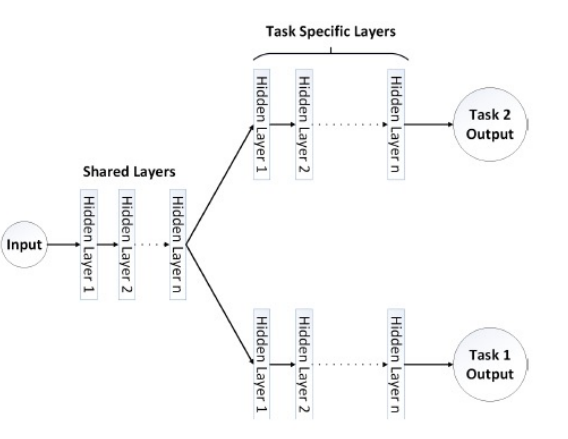
\includegraphics[width=0.5\textwidth]{img/multitask.png}
    \caption{Multitasking learning}
    \label{fig:multitask}
\end{figure}
\begin{note}
    Multitasking learning is a form of parameter sharing.
\end{note}

Shared parameters improve generalization in proportion of number of examples for
the general task. Additional task imposes constraints on the parameters in the
shared layers preventing overfitting.
\begin{note}
    Improvement in generalization only occurs when there is something shared across
    the tasks at hand.
\end{note}
\subsubsection{Early stopping}
When training large models with sufficient representational capacity to overfit
the task, we often observe that training error decreases over time but validation
error begins to rise again. We can obtain a model with better validation error by
returning to the parameter setting at the point in time with the lowest validation
error.

\textbf{Early stopping} is one of the most common techniques used. We can think
at this technique as a hyperparameter selection method, where training time is
the hyperparameter to be chosen.

Early stopping can be implemented as follow:
\begin{enumerate}
    \item Choose number of iterations $n$
    \item Train model for $n$ iterations
    \item Validate model and compute validation error, compare consecutive validation
          error and return to point 2 until delta is insignificant or negative.
\end{enumerate}
Every iteration model improves its weights until it starts to going in overfitting.
\begin{note}
    It's impossible to write all parameters on disk during training.
\end{note}
\begin{figure}[!ht]
    \centering
    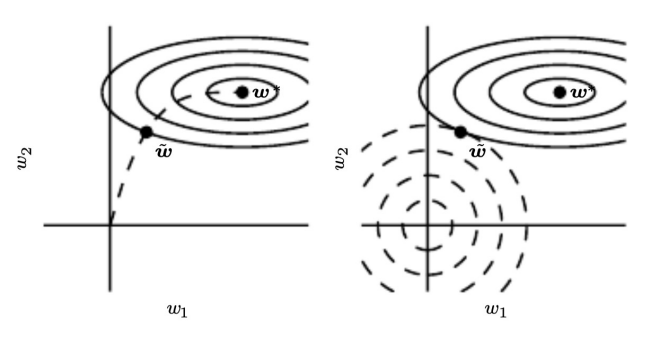
\includegraphics[width=0.5\textwidth]{img/early_stopping.png}
    \caption{On the left we can see the process of early stopping, while on the
        right we can see a classic regularization process.}
    \label{fig:earlystopping}
\end{figure}
\subsubsection{Parameters Tying}
\textbf{Parameters Tying} refers to explicitly forcing the parameters of 2 models
to be close to each other using the norm penalty:
\begin{equation}
    \|w(A)- w(b)\|
\end{equation}
with $A$ and $B$ respectively first and second model. This norm penalty is added
to the objective function like a constraint. It is used in Siamese networks,
convolution operators and multitasking learning.
\subsubsection{Bagging}
\textbf{Bagging} is a technique for reducing generalization error combining
several models (\textbf{ensemble model}).

You have to train $k$ different models on $k$ different subsets of training data
with same number of examples as original dataset using a random sampling with
replacement.

Every model is then tested, they produce $k$ votes for the final result. These
models are called ensemble.

The objective of this method is to introduce generalization by using different
models trained on different examples using different initialization hyperparameter
and different structures to have independent errors.

Cons of this method is that ensemble models doesn't provide us a scalable way to
improve performance, moreover we have 2-3 models inside the ensemble.
\subsubsection{Dropout}
\textbf{Dropout} provides a computationally inexpensive but powerful method of
regularizing a broad family of models. It provides an inexpensive approximation
of a ensemble with a high number of sub-networks of the starting one.

All the sub-networks should be formed by removing non-output units from underlying
base network, generating an exponential number of models, using a treatable
amount of memory.

This technique eliminates the need to accumulate model votes in the inference
phase. It is intended to train the model to be learned by switching on and off
with different probabilities input neurons or neurons in the hidden layers.

To do a train phase we use a \textbf{minibatch-based learning algorithm} that
makes small steps, such as stochastic gradient descent.

Each time we change minibatch we \textbf{randomly sample} a different binary mask
to apply to all input and hidden units in the network. Typically the distribution
use for sampling is not uniform. For example, the probability of keeping a hidden
unit is $0.5$, while the probability of including an input unit is $0.8$.

We can have some problem, indeed, at training time we are required to divide the
output of each unit by the probability of that unit's dropout mask, so we assign
as likelihood on the output. In this way we make sure that the expected total
input to a unit at test time is the same as the expected total input of that unit
at train time.

We haven't theoretically basis for the accuracy but empirically it perform well.
Complexity of dropout is limited to a $\mathcal{O}(n)$ computation per example
to update because it needs to generate a total of $n$ random numbers and multiply
them by the state.

Dropout can be used with every model and also with stochastic gradient descent.
The cost of applying dropout to the entire model could be significant, but the
amount of benefit on generalization error couldn't be enough to the cost of the
regularization.
\subsubsection{Adversarial training}
We can add \textbf{adversarial examples} (inputs perturbed by noise) to train the
model for robustness. These are used to train the network and will allowed us to
reduce test errors.

Adversarial examples can be generated by adding to a bit of perturbation on some
train example with a low multiplication factor of noise. This method allowed us
to generate new examples for training from the original train set with slightly
changes that are unrecognized by humans.
\section{Generative Adversarial Models}
\textbf{Generative Adversarial Network} (GAN) are generative model that
implicitly learn the \textbf{data distribution} from a zero-sum game between 2
computing neural network:
\begin{itemize}
    \item \textbf{Discriminator}: a neural network that classify examples between
          fake and real.
    \item \textbf{Generator}: generate fake example that are given as input to the
          discriminator.
\end{itemize}

\begin{figure}[!ht]
    \centering
    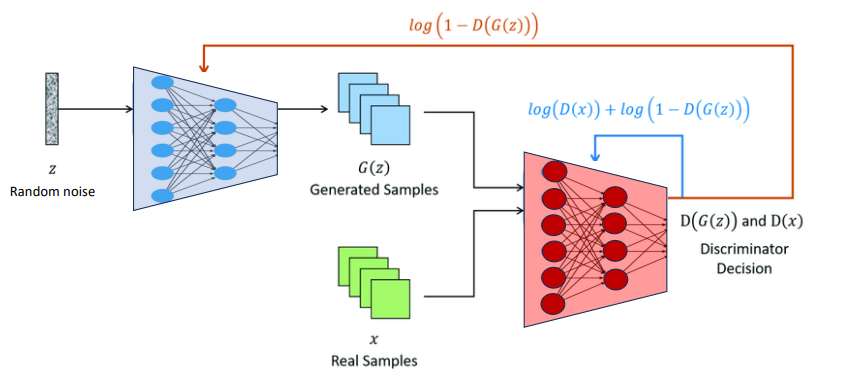
\includegraphics[width=0.5\textwidth]{img/GAN.png}
    \caption{Generative Adversarial Network}
    \label{fig:gan}
\end{figure}

The target of the generator is to generate example the most similar to real one
in such a way to be classified in real example by the discriminator. Quite the
opposite the discriminator have to identify real examples from fake one. If the
discriminator makes a mistake so we will update discriminator's weights, vice
versa we will update generator's weights.
\section{Optimization for training deep models}
When we are creating a deep learning model, we have to consider different aspects
to optimize the training process. In this section, we are going to see some
issues that can arise during the training process and how to solve them.

Let's start by introducing the difference between \textbf{optimization} and
\textbf{machine learning}. In the first case, we are trying to minimize a function
acting directly on it, while in the second case we are trying to minimize a loss
function that is a proxy for the true function we want to minimize.

In machine learning, we aim to optimize a performance measure $P$, based on the
test set. This is done by optimizing a different function $J(\theta)$, with the
hope that improvements in $J(\theta)$ lead to improvements in $P$.

Typically, the loss function is a simple average over the training set and can be
written as:
\begin{equation}
    J(\theta) = E_{(x, y) \approx \hat{P}_{data}} \mathcal{L}(f(x, \theta), y)
\end{equation}
where $\mathcal{L}$ is the loss function, $f$ is the model, $x$ is the input, $y$
is the target and $\theta$ are the parameters of the model. Also, $\hat{P}_{data}$ is
the empirical distribution of the data.

If we know the true data distribution $P_{data}$, the loss function, also called
the \textbf{risk function}, can be expressed as:
\begin{equation}
    J(\theta) = E_{(x, y) \approx P_{data}} \mathcal{L}(f(x, \theta), y)
\end{equation}
and this reduce the machine learning problem to an optimization problem.

The problem of using the empirical distribution is that the model is prone to
overfitting, because we don't have enough data to represent the real distribution.

Instead of minimizing the empirical risk, we can minimize a \textbf{surrogate
    loss function}. This function is a proxy for the true loss function and it
is easier to optimize.

Another difference is that training algorithms doesn't halt at local minima, but
when the early stopping criterion is met. This can be roughly thought of as a
way to reincorporate the true loss function in the learning process.
\subsection{Batch and Minibatch}
One aspect of machine learning algorithms that separates them from general
optimization algorithms is that the objective function usually decomposes as a
sum over the training examples. Computing this expectation exactly is very
expensive, since it requires evaluating the model on every example in the entire
dataset.

However, we can compute these expectations by randomly sampling a small number
of examples from the dataset at every iteration. This works because we are
computing an expected value and, the \textbf{standard error} of the mean estimated
from a sample of size $m$ is:
\begin{equation}
    SE(\mu) = \sqrt{VAR\left[\frac{1}{m}\sum x^{(i)}\right]} = \frac{\sigma}{\sqrt{m}}
\end{equation}
where $\sigma$ is the standard deviation of the distribution. This equation shows
that the relationship is sub-linear between the number of examples and the standard error.

Another consideration that motivates the estimation of the gradient from a
small number of samples is the redundancy in the training set.

Optimization algorithms that use the entire training set to compute the gradient
are called \textbf{batch} or \textbf{deterministic gradient methods}. While the
ones that use a single training example for that task are called \textbf{stochastic
    gradient methods}. Most of the algorithms we use for deep learning fall
somewhere in between and they are called \textbf{mini-batch} or \textbf{mini-batch
    stochastic methods}. We can see the difference between these methods in the
following figure \ref{fig:batchminibatch}.

\begin{figure}[!ht]
    \centering
    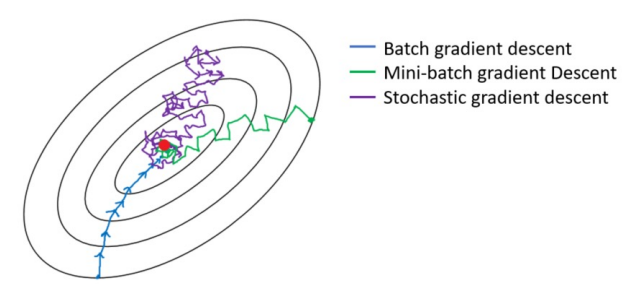
\includegraphics[width=0.5\textwidth]{img/minibatchvsbatch.png}
    \caption{Difference between batch, mini-batch and stochastic gradient methods.}
    \label{fig:batchminibatch}
\end{figure}

In order to chose the right size of the mini-batch, we have to consider that a
larger size will provide a more accurate estimate of the gradient, but with less
than linear improvement in the standard error. While a smaller size will provide
a less accurate estimate of the gradient, but with more than linear improvement
in the standard error and doesn't use the full computational power of the GPU.

\begin{note}
    Usually, a good choice is a power of 2.
\end{note}

It is extremely crucial that mini-batches are sampled at \textbf{random}, because
computing an unbiased estimate of the expected gradient from a set of samples
requires that those samples be independent.

When the order of elements in the dataset holds some significance, it is absolute
necessity to shuffle the examples before selecting every mini-batch.
\subsection{Challenges in deep learning}
Traditionally, machine learning has avoided this difficulty by carefully designing
the objective function and constraints to insure the problem is convex. However,
for training deep models we usually face non-convex optimization.
\subsubsection{Ill-conditioning}
The first challenge is \textbf{ill-conditioning}. This is a problem that arises
when the optimization problem is poorly conditioned. This means that the curvature
of the loss function is very different in different directions.

This condition manifests in stochastic gradient descent when small steps increase
the loss function.

This problem can be identify by looking at the \textbf{condition number} of the
Hessian matrix. If the condition number is very large, we have an ill-conditioned
problem.
\begin{figure}[!ht]
    \centering
    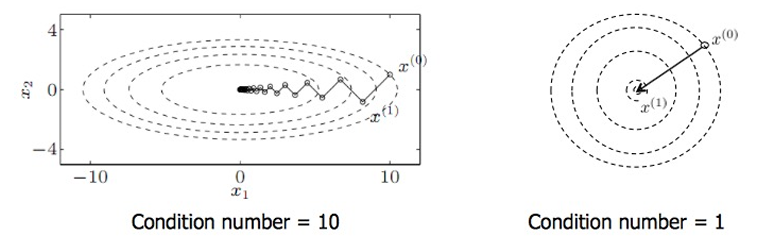
\includegraphics[width=0.5\textwidth]{img/illConditioned.png}
    \caption{Ill-conditioning}
    \label{fig:illconditioning}
\end{figure}

\subsubsection{Local minima}
Functions involved in deep models are guaranteed to have an extremely large
number of local minima. However, we will see that local minima are not
necessarily a major problem because plateaus are an acceptable solution.

Neural networks aren't \textbf{identifiable} there is no single set of parameters
from a single training set. In fact, if we have $m$ layers with $n$ neurons each,
there are $n!^m$ ways to arranging the hidden units to obtain equivalent solutions.
This is called \textbf{weight space symmetry}.

Model identifiability issues mean that there can be an extremely large or even
uncountably infinite amount of local minima in the cost function of deep models.
However, these local minima are all equivalent in value and are not a problematic
form of non-convexity.

Local minima are only truly problematic if they have a much higher cost than the
global minimum.
\subsubsection{Saddle points}
For many high-dimensional non-convex functions, local minima and maxima are in
fact rare compared to \textbf{saddle points}.

A saddle point is a point where the Hessian matrix has both positive and negative
eigenvalues and the gradient is zero. We can think of a saddle point as being a
local minimum along one cross-section of the cost function and a local maximum
along another.

\begin{figure}[!ht]
    \centering
    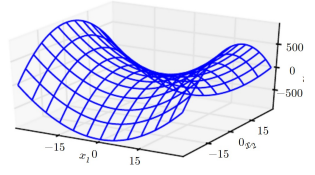
\includegraphics[width=0.5\textwidth]{img/saddle.png}
    \caption{Saddle point}
    \label{fig:saddle}
\end{figure}

This points are more common in high-dimensional spaces than local minima and they
are a problem for optimization algorithms because they are points where the gradient
is zero but they are not a minimum.

For first-order optimization algorithms that use only gradient information, the
situation is unclear. The gradient can often become very small near a saddle point.
On the other hand, gradient descent empirically seems to be able to escape saddle
points in many cases. While, for Newton's Method, saddle points constitute a
major problem, because it actively seeks solutions at critical points where the
gradient is zero.
\subsubsection{Plateaus}
Another problem that can arise during the training process is the presence of
\textbf{plateaus} or \textbf{flat regions}. These are regions where the gradient
is very small and the optimization algorithm can't make progress.
\subsubsection{Cliffs and exploding gradients}
Neural networks with many layers often have extremely steep regions reassembling
cliffs. This regions are the result from the multiplication of many large weights
together.

An extremely steep cliff structure, the gradient update step can move the
parameters extremely far, usually jumping off of the cliff structure altogether.

A solution to this is to use the \textbf{gradient clipping heuristic} which
intervenes to reduce the step size to be small enough that it is less likely to
go outside the region where the gradient indicates the direction of approximately
steepest descent.
\subsubsection{Additional Problems}
There are other problems that can arise during the training process, such as:
\begin{itemize}
    \item \textbf{Long Term Dependencies}: arises when the computational graph
          is very deep. The result of this problem is vanishing and exploding
          gradients.
    \item \textbf{Inexact Gradients}: we usually only have a noisy or even biased
          estimate of the gradient and the Hessian. Sometimes, gradients for our
          loss functions are even intractable. Not a big issue in neural network
          training. Surrogate loss functions tend to perform well enough in practice.
    \item \textbf{Poor Correspondence between Local and Global Structure}: it is
          possible to overcome all of the above problems at a single point and
          still perform poorly if the direction that results in the most
          improvement locally does not point toward distant regions of much
          lower cost.
\end{itemize}
\begin{note}
    The initialization is very important.
\end{note}
\subsection{Optimization algorithms}
There are many optimization algorithms that can be used to train deep models.
In this section, we are going to see some of them.
\subsubsection{Stochastic Gradient Descent}
\textbf{Stochastic Gradient Descent} (SGD) is the most used optimization algorithm
in deep learning. It is based on the idea of computing the gradient of the loss
function on a mini-batch and then update the weights of the model. We can describe
the algorithm as follows:
\begin{itemize}
    \item Sample a mini-batch of examples from the training set.
    \item Compute the gradient of the loss function on the minibatch.
          \begin{equation}
              g \gets \frac{1}{m} \nabla_\theta \sum_{i=1}^m \mathcal{L}(f(x^{(i)}; \theta), y^{(i)})
          \end{equation}
    \item Update the weights of the model using the gradient.
          \begin{equation}
              \theta \gets \theta - \epsilon_k g
          \end{equation}
\end{itemize}
It is important to note that the learning rate $\epsilon_k$ is a hyperparameter
that must be adaptive. This is because the learning rate is a very important
hyperparameter and it can affect the convergence of the algorithm. A sufficient
condition for convergence is:
\begin{equation*}
    \sum_{k=1}^\infty \epsilon_k = \infty \quad \text{and} \quad \sum_{k=1}^\infty \epsilon_k^2 < \infty
\end{equation*}

A common way to implement an adaptive learning rate is to use a linear decay
until the iteration $\tau$. This can be done as follows:
\begin{equation}
    \epsilon_k = \left(1 - \alpha\right)\epsilon_0 + \alpha \epsilon_\tau
\end{equation}
In this case we have to choose three hyperparameter: $\epsilon_0$, $\epsilon_\tau$
and $\alpha$. Usually, $\epsilon_\tau$ is chosen to be $1\%$ of $\epsilon_0$.

To choose $\epsilon_0$ we can try to make different run for a fixed number of
iterations and choose the best one.
\subsubsection{Momentum}
\textbf{Momentum} is a method that helps accelerate SGD in the relevant direction
and dampens oscillations. It is a method that accumulates an exponentially decaying
average of past gradients and continues to move in their direction.

The update rule for momentum is:
\begin{equation}
    \theta \gets \theta + v
\end{equation}
where $v$ is the velocity vector and it is defined as:
\begin{equation}
    v \gets \alpha v - \epsilon \frac{1}{m} \nabla_\theta \sum_{i=1}^m \mathcal{L}(f(x^{(i)}; \theta), y^{(i)})
\end{equation}
where $\alpha$ is the momentum parameter and it is usually set to $0.9$.

This algorithm aims to solve the problem of poor conditioning of the Hessian
matrix, and the variance of stochastic gradients.

The momentum algorithm can be seen as a ball rolling down a hill. The ball
gathers momentum as it rolls down the hill, and it continues to move in the
direction of the momentum even if it encounters a small hill.
\subsubsection{Delta Bar Delta}
\textbf{Delta Bar Delta} is a method that adapts the learning rate for each
parameter. It is based on the following idea:
\begin{itemize}
    \item if the partial derivative of the loss function with respect to a
          parameter remains the same, increase the learning rate.
    \item otherwise, if that partial derivative changes sign, decrease
          the learning rate.
\end{itemize}
\subsubsection{AdaGrad}
\textbf{AdaGrad} is a method that adapts the learning rate for each parameter.
This method scale the gradient according to the historical norms. In this way,
learning of parameters with high partial derivatives decrease faster.

This method is based on the following idea:
\begin{itemize}
    \item Accumulate the square of the gradient into a vector $r$.
          \begin{equation}
              r \gets r + g \odot g
          \end{equation}
    \item Update the weights element wise.
          \begin{equation}
              \Delta\theta \gets - \frac{\epsilon}{\sqrt{r + \epsilon}} \odot g
          \end{equation}
    \item Update parameters
          \begin{equation}
              \theta \gets \theta + \Delta \theta
          \end{equation}
\end{itemize}
\subsubsection{RMSProp}
\textbf{RMSProp} is a method that adapts the learning rate for each parameter.
This method is a modification of AdaGrad to perform better on non-convex problems.
The main difference is that RMSProp use an exponentially weighted moving average.
This method is based on the following idea:
\begin{itemize}
    \item Accumulate the square of the gradient into a vector $r$.
          \begin{equation}
              r \gets \rho r + (1 - \rho) g \odot g
          \end{equation}
    \item Update the weights element wise.
          \begin{equation}
              \Delta \theta \gets - \frac{\epsilon}{\delta + \sqrt{r}} \odot g
          \end{equation}
    \item Update parameters
          \begin{equation}
              \theta \gets \theta + \Delta \theta
          \end{equation}
\end{itemize}
\subsubsection{Adam}
\textbf{Adam} is a variation of RMSProp in which we add the momentum. Also, it
add a bias correction to the moments to account for their initialization at the
origin. This method is based on the following idea:
\begin{itemize}
    \item Update time step:
          \begin{equation}
              t \gets t + 1
          \end{equation}
    \item Update biased moment estimates
          \begin{equation}
              \begin{split}
                  s \gets & \rho_1 S + (1 - \rho_1)g          \\
                  r \gets & \rho_2 r + (1 - \rho_2) g \odot g
              \end{split}
          \end{equation}
    \item Correct biases
          \begin{equation}
              \begin{split}
                  \hat{s} \gets & \frac{S}{1 - \rho_1^t} \\
                  \hat{r} \gets & \frac{r}{1 - \rho_2^t}
              \end{split}
          \end{equation}
    \item Update parameters
          \begin{equation}
              \Delta \theta \gets - \epsilon \frac{\hat{s}}{\delta + \sqrt{\hat{r}}}
          \end{equation}
    \item Update model params:
          \begin{equation}
              \theta \gets \theta + \Delta \theta
          \end{equation}
\end{itemize}